% Information and metadata
% --------------------------

	\newcommand{\ccourse}{BADM500}							% \ccouse - course code (and name)
    \newcommand*\xor{\oplus}

% Preamble
% --------------------------
	% BEGIN_FOLD

	% Document Setup
	% ------------------------
	\documentclass[11pt,a4paper]{article}       		% Optional = twoside for two-sided documents

	% Packages
	% ------------------------
		% BEGIN_FOLD

			% Essential Packages
			\usepackage[english]{babel}					% Language pack
			\usepackage[utf8]{inputenc}					% Input encoding for UTF8

			% Mathematics Packages
			\usepackage{amsmath}						% Basic math tools
			\usepackage{amssymb}						% Basic math symbols

			% Programming Packages
			\usepackage{listings}						% Listings provide code environments
			\usepackage{courier}						% Font package for code

			% Layout Packages
			\usepackage{lastpage}
			\usepackage{graphicx}						% Importing .svg, .pdf and other
			\usepackage{caption}						% Custom figure captions
			\usepackage{fancyhdr}						% Package for fancy headers and footers
			\usepackage{float}							% Float options for placing images, tables, etc.
			\usepackage{courier}						% Courier font for code
			\usepackage{subcaption}						% Separate captions for subimages
			\usepackage{color}                          % Gives colour commands (Used for links)
			\usepackage[pdftex, colorlinks]{hyperref}   % Makes hyperlinks work and coloured
			\usepackage[paperwidth=8.5in]{geometry}     % Enlarges the width of the page by inches
			\usepackage[noabbrev,capitalize]{cleveref}
			\usepackage{dirtree}

			% Drawing and diagram packages
			\usepackage{tikz}							% Package for drawing diagrams

			% Misc. Packages
            \usepackage{nameref}                        % Package for referencing names
            \usepackage{leading}                        % Package for giving the lines spacing
            \usepackage{comment}                        % Allows to comment entire paragraph
            \usepackage{tabularx}
            \usepackage[ruled,vlined]{algorithm2e}
            \usepackage{url}
            

		% END_FOLD

	% Shortcuts and commands
	% ------------------------
		% BEGIN_FOLD
  			\newcommand{\code}[1]{\lstinline|#1|}							% \code{} Insert code here to have in-line code.
			
			\newcommand{\br}{\newline\newline}                              % Adds an empty line


		% END_FOLD

	% Settings / Preferences
	% ------------------------
		% BEGIN_FOLD

			% Equation, align, and gather environments can have page breaks
			\allowdisplaybreaks

			% Coloured links (Optional, delete for non-coloured links)
			\hypersetup{colorlinks,
				citecolor = black,
				filecolor = black,
				linkcolor = black,
				urlcolor = blue
				}

			% Colours for code environment
			\definecolor{codegreen}{rgb}{0,0.6,0}
			\definecolor{codegray}{rgb}{0.5,0.5,0.5}
			\definecolor{codepurple}{rgb}{0.58,0,0.82}
			\definecolor{backcolour}{rgb}{0.95,0.95,0.92}

			% Configure code environment
			\lstset{
				numbers			= left,
				stepnumber 		= 5,					% Numbers every 5 lines of code
				firstnumber 	= 1,
				numberfirstline = true,
				showtabs 		= false,
				basicstyle		= \ttfamily,
				breaklines		= true,
				columns			= fixed,
				showspaces		= false,
				commentstyle	= \color{codegreen},
				keywordstyle	= \color{magenta},
				numberstyle		= \color{codegray},
				stringstyle		= \color{codepurple},
				showstringspaces= false
				}

			% Nicer dots for itemisation
			\renewcommand{\labelitemi}{·}				% Nicer dots for 'itemize' environments

            
		% END_FOLD

	% END_FOLD

% Layout (Header and footer can be edited here)
% --------------------------
	% BEGIN_FOLD

		% Margins
		\addtolength\textheight{2cm}
		\addtolength\topmargin{-1cm}
		\addtolength\marginparwidth{1.5cm}
		\addtolength\headheight{1.6pt}

		% Indent and paragraphs
		\setlength\parindent{0pt} 								% Comment to indent first line in  paragraph
		
		% Line spacing
		\leading{17pt}

		% Header, footer
		\pagestyle{fancy}										% Template for header and footer
		%\fancyhf{}												% Set header and footer to empty

		% Left header (inner if using twopage layout)
		\fancyhf[HLO]{University of Southern Denmark}

		% Center header
		\fancyhf[HC]{\ccourse}

		% Right header (outer)
		\fancyhf[HRO]{01-06-2021}

		% Left footer (inner)
		%\fancyhf[FLO,FRE]{}

		% Center footer
		\fancyhf[FC]{Page \thepage \, of \pageref{LastPage}}

		% Right footer (outer)
		%\fancyhf[FRO,FLE]{}

	% END_FOLD
	
% ==========================
% Document
% ==========================
\begin{document}

% 	\maketitle 													% Prints title, author and date
% 	\begin{minipage}[t]{0.6\textwidth}
%         \begin{flushleft} \large
%             \emph{Author:}\\
%             \text{Mikkel Juul Vestergaard}
%         \end{flushleft}
%     \end{minipage}
%     \begin{minipage}[t]{0.4\textwidth}
%         \begin{flushright} \large
%             \emph{Supervisor:} \\
%             \text{Assist. professor,}\\
%             \text{Ruben Niederhagen}
%         \end{flushright}
%     \end{minipage}\\[3cm]

    \begin{titlepage}
    \begin{center}
        \vspace*{1cm}
            
        \LARGE
        \textbf{Post Quantum Cryptography on the RISC-V Platform - Rainbow}
            
        \vspace{2cm}
        
        \Large
        \emph{Author:}\\
        Mikkel Juul Vestergaard
        
        \vspace{0.5cm}
        \emph{Supervisor:}\\
        Assist. Professor Ruben Niederhagen
        
        \vspace{0.5cm}
        \emph{External censor:}\\
        Associate Professor Claudio Orlandi
        
        \vspace{1cm}
        \emph{Project Repository:}\\
        \url{https://github.com/Moggel12/Riscv-Rainbow}
        \vfill
        
        \vspace{0.8cm}
            
        
\includegraphics[width=0.6\textwidth]{resources/SDU.jpeg}
            
        \Large
        Department of Mathematics and Computer Science\\
        University of Southern Denmark\\
        Denmark\\
        01-06-2021
            
    \end{center}
\end{titlepage}


    %
\includegraphics[width]{resources/SDU.png}
    \thispagestyle{empty}% No header or footer on first page
    \pagenumbering{gobble} 
   	%\thispagestyle{fancy}										% First page with header and footer
    \newpage
    \thispagestyle{empty}
    \tableofcontents %Indholdsfortegnelse

    \newpage
    \pagenumbering{arabic} 
    \nocite{*}
    % Include new tex files here.
    % --------------------------
        \section*{Resumé}
I denne rapport, og dette projekt generelt, bliver en RISC-V implementering af Rainbow signatur systemet fremlagt. Rainbow er en finalist i NIST standardiseringsprocessen for \emph{post-quantum} kryptografiske algoritmer i kategorien for digitale signatur systemer. Den overførte version af reference implementeringen vil blive gennemgået og testet for antallet af CPU cyklusser og instruktioner. Grundlaget for projektet var derfra at opnå kendskab til \emph{post-quantum} kryptologi, med særligt fokus på Rainbow, samt at give potentielle optimeringer til systemet med CPU cyklusser og instruktioner i fokus.
\medskip\\
De optimeringer der blev forsøgt implementeret til Rainbow inkluderede \emph{bitslicing} og \emph{opslagstabeller}. Ingen af disse to optimeringer formåede at opnå et lavere antal cyklusser end standard (reference) implementeringen (efter at være oversat til RISC-V platformen). Dog opnåede \emph{bitslicing} systemet en bedre cykel/instruktion-ratio end de to andre versioner (\emph{opslagstabeller} og reference) til trods for et markant større antal cyklusser. Antallet af cyklusser i den pågældende version for bitslicing nåede 3300\% flere end standard implementering. Til trods for dette, står denne bitslicing variant som et \emph{fundament} til at afprøve yderligere optimeringer, særligt på \texttt{C}-kode i et højere niveau, med relation til bitslicing.

\pagebreak
        \section{Introduction}
The modern world of computing has grown to become a largely impactful aspect of everyones lives. Due to this increasing impact it is not uncommon for perpetrators to attack the digital structures that societies rely on. Whether it is against personal computing or more societally important computing functions, some seek to abuse the importance of modern day computing for financial, activist, or other types of gain.\medskip\\
As the rise of the public internet, connecting billions of people and organizations, made this even more prominent and easy for perpetrators to abuse, cryptologists, mathematicians and computer scientists all over have tried to minimize the risk of using a public internet of computing for important tasks like banking, business confidentials, personal health, etc.\medskip\\
The main aspects of this digital cryptology are public-key cryptography, symmetric-key cryptography and hashing. These three aspects each play their different roles in securing the lives and information of billions of people globally. Depending on the information and computing power available, these will be used for different purposes, as they each provide their own unique take on private life on the public internet.\medskip\\
For securing sensitive information from external readers, symmetric key algorithms or public-key algorithms are typically used. A symmetric-key encryption scheme is fast and typically has small key-sizes, though it relies on both parties knowing the key in advance. A public-key scheme allows communicating parties to exchange public keys and encrypting data to eachother through these, typically sacrificing speed and key-sizes.\medskip\\
For storing passwords and other personal information it is typical to use hashing as a one-way "encryption" of data, such that only the user itself knows what this information is. Hashing can also be used to verify the authors of certain publicly shared documents, by incorporating public-key schemes into the mix and therefore enabling anyone to use a mixture of a public-key encryption and hashing to digitally sign a document.\medskip\\
As researchers world-wide constantly look for new ways of computing, like DNA computing, photonic computing, quantum computing, and more, the cryptographic strength of standardized in-use cryptographic algorithms has also been challenged. The strengths of some modern computing-types like quantum computing over standard electrical computers have shown their ways into the cryptographic scene.\medskip\\
Algorithms like RSA and Diffie-Helmann key-exchange, standard and elliptic-curve, are both well-known cryptographic algorithms that will become obsolete once sufficiently strengthed quantum computers become less rare. Currently many big tech-companies are working on quantum computers, and the strength of each is ever increasing.\medskip\\
A quantum computer computes quite differently from a standard computer, as it uses \emph{qubits} instead of the more well-known \emph{bits}. As many might be aware of, a standard computer works by having a central processing unit and some storage local to it, some persistent and some not. The central processing unit works, on a virtual scale, by using values of 0s and 1s to determine its actions and as the values that these actions act upon.\medskip\\
A quantum computer, and the qubits that it works with, does not consider either a 0 or a 1 value whenever it reads some qubits. The qubits can be implemented using electrons or photons. The idea of quantum computing is then to harness aspects of quantum physics, such as using superposition to have qubits represent multiple combinations of 0s and 1s at the same time, whereas a typical computer would have a string of bits be a single combination. Due to such aspects as superposition, entanglement and decoherence, sufficiently-sized quantum computers have been proven to provide a significant speedup in some problems over standard electrical computers, some of which relate to the security of modern day cryptographic algorithms.\medskip\\
Although such computers might seem like they would have to replace standard electrical computers, the current state of cryptography is to build cryptographic schemes that are secure against quantum computers, but can still be ran on a typical personal computer without significant disadvantage. These algorithms, also called \emph{post-quantum cryptographic algorithms}, have been under a standardization process by NIST for a few years, by 2021.\medskip\\
As quantum computers are not here to replace every typical electric computer in use, the global technology market has to adapt products to use these \emph{post-quantum} algorithms. One such market is the IOT, or Internet Of Things, market. IOT devices are gradually more and more normal to see in everyday-homes and therefore must also follow this security trend. Though, the problem with IOT devices is that they typically have to run low power-consumption hardware with small computational footprints. As it is inevitable that most post-quantum cryptographic algorithm are not made directly for IOT hardware it can be quite a lot heavier to run post-quantum tasks on IOT hardware, meaning that more localized optimizations for IOT and embedded hardware implementations is in need.\medskip\\
IOT devices are also not the only aspect of the technology market that is in need for such small processors. Modern vehicles, mobile phones, tablets, laptop computers, home appliances, robot- and drone controllers, and more, all require small low power-consuming processing units for providing their core functionalities.
\pagebreak
        \section{Preliminaries}
In subsection \ref{rainscheme} a general overview of the Rainbow Signature scheme, and the necessary theory and terminology, is given. In subection \ref{pre-riscv} we seek to briefly explain the nature of Reduced Instruction Set Computers and the processing utility used for running this project.
\subsection{The Rainbow scheme} \label{rainscheme}
The Rainbow cryptographic scheme is a multivariate public key cryptosystem (MKPC) that stands as a round 3 candidate in the NIST post-quantum standardization for signature schemes. Being an MKPC, a central aspect of Rainbow is the $NP$-completeness of solving multivariate polynomial systems, or more specifically multivariate quadratic, $MQ$, systems which is given as the NP-hard MQ-problem. [Multivariate public key cryptosystem chapter 2]
\medskip\\
The internal workings of MKPCs, in general, make use of a public key consisting of various nonlinear multivariate quadratic, MQ, polynomials defined over some finite field. According to the security level chosen for Rainbow the field sizes adjust, meaning that the variants of Rainbow are 
\begin{itemize}
    \item Level I security: Defined over $GF(16)$
    \item Level III security: Defined over $GF(256)$
    \item Level V security: Defined over $GF(256)$
\end{itemize}
with $GF$ being a Galois field, in this case $GF(2^q)$ with $q = 4$ or $q=8$. The above security levels encapsulate one or more of the NIST-specified security levels (I, II, III, IV, V). In addition to having three security levels, the rainbow scheme also has three variations. These variations correspond to the way the algorithm handles keys, to provide smaller key sizes sacrificing speed in some cases. [NIST rainbow round 3 paper]\medskip\\
As was earlier noted, the keys of Rainbow consist of maps. Specifically, with $n$ variables and $m$ equations, the public key is a mapping $\mathbb{F}_q^n \rightarrow \mathbb{F}_q^m$. The \textit{public key} $P = S \circ F \circ T$ is the composition of three maps. The maps $S$ and $T$ are affine invertible maps used to hide the structure of the central map $F$. The central map $F$ is an invertible map consisting of $m$ multivariate polynomials in $n$ variables. These polynomials are given over various layers of the Oil and Vinegar scheme, also called the \textit{Rainbow layers}. The \textit{secret key} consist of $S$, $F$ and $T$ indivudally.[Multivariate public key cryptosystem chapter 5]\medskip\\
To compute and verify signatures using Rainbow, the maps are used in different ways.
For \textit{signature generation}, the algorithm uses the invertibility of the three maps of the secret key and a hash function to generate signatures. In broad terms, the signature generation scheme uses the hashed document, say $\mathbf{w}$, as input into $\mathbf{x} = S^{-1}(\mathbf{w}), \mathbf{y} = F^{-1}(\mathbf{x}), \mathbf{z} = T^{-1}(\mathbf{y})$, with $F^{-1}(\mathbf{x})$ being some suitable pre-image of $\mathbf{x}$ under $F$. The \textit{signature verification} scheme is quite simpler, as it for some hash function $H$, document $d$, and public key $P$ checks if $P(z) = H(d)$ which has to hold for it to accept.[Multivariate public key cryptosystem chapter 5]

\subsection{The RISC-V ISA} \label{pre-riscv}
Architectures in modern computing fall in to one of two categories, Reduced Instruction Set Computers (RISC) or Complex Instruction Set Computers (CISC). A RISC machine seeks to reduce on the complex nature of certain aspects of CISC machines, as CISC machines have been growing in complexity following the rise of high-level langauges like Java, Python, etc. RISC architectures are typically optimized with regard to register use (either through the compiler or through having an adequate amount of actual hardware registers), instruction pipelines, and having small and fewer instructions (compared to Complex Instruction Set Computer architecture). The optimizations mentioned above came about as multiple studies showed operand referencing, conditional branches, procedure calls and predictable, and small, instruction costs were of importance when looking at how high-level languages interacted with low-level assembly and machine code. [William Stallings, chapter 15] \medskip\\
One such RISC architecture is the RISC-V architecture. RISC-V is an open standard and as such can be freely implemented for different kinds of usage. Any RISC-V implementation is supposed to be some combination of the base RISC-V ISA, which is limited but still usable for many general purposes, and optional extensions providing features like atomic instructions, multiplication and division, floating point support and more. A subset of the extensions and their base ISAs can be seen in [RISC-V Offers Simple, Modular ISA] or [Design of the RISC-V Instruction Set Architecture].
\medskip\\
For this project, the processor used for benchmarking is a VexRiscV-based platform called PQVexRiscV simulated, on a logical level, on a host machine running a Ryzen 7 5800X. Simulating on a logical level, in contrast to a functional level, has the benefit that cycle counts are accurate and therefore can be used for benchmarking as well. The CPU being simulated will be ran with \texttt{512kB} of RAM and equivalently for ROM. The CPU is openly available and was originally created for the \texttt{pqriscv} project, the RISC-V counterpart to the \texttt{pqm4} library [PQVexRiscV reference]. The VexRiscV CPU in general is an RV32IM instruction set CPU, meaning that it has the 32-bit integer base ISA with the multiplication and division extensions, running a five stage pipeline (fetch, decode, execute, memory, writeback). The VexRiscV CPU is optimized for FPGA use [VexRiscV docs] and as such is interesting with regard to embedded or industrial use (for now at least). Other than usage of the PQVexRiscV CPU this project is not affiliated with the \texttt{pqriscv} project nor the \texttt{VexRiscV} project. Although some newer in-progress extensions for RISC-V might be in the works, this project will be working from the RV32IM instruction set used by the VexRiscV CPU by default.\medskip\\
        \section{Implementation}
The following sections detail the differences that came about when porting the reference implementation \cite{rainbowgit} to a platform without an operating system, minimal standard library, and more constrained on memory. It will also detail some of the specifics that the original authors used to implement the functionality of Rainbow for reference in later sections. It will, however, not go into detail on how the optimizations tested differ from the original code, see \cref{opti} for this.
\medskip\\
The files and functionality gone through in this section are what is left from porting the implementation to RISC-V. If any changes were made to a file or functionality from the original code it will be described in of the following subsections.
\subsection{Overview of the Reference System}
In general, this port of the Rainbow reference implementation tries to stay as close to its roots as possible, making it easier to argue for correctness and easier to port these findings to other platforms as well (having multiple sources being somewhat similar).
\medskip\\
The variant worked on for this project is solely the standard Rainbow variant with no key-size adjustments and a security level of I. Focusing on this particular variant of the Rainbow scheme makes the optimizations done clearer for readers new to the Rainbow scheme in general, as it is the closest to how Rainbow is described in many sources on Rainbow and the $MQ$ problem and therefore should be somewhat easier than also having to understand some of the key-size reductions going on in \texttt{CZ-Rainbow} and \texttt{Compressed-Rainbow}.
\subsubsection{File Overview}
The files of the reference implementation can be divided into different parts according to what aspect of the Rainbow scheme they partake in. In total, we give an overview of the functionality of this Rainbow port by dividing into these parts and explaining each part separately. First we give an overview of the files in \texttt{src/Ia\_Classic\_Reference}.
\medskip\\
One set of files of this port that had to have quite a lot of changes made to it was the files prepended with \texttt{utils}. These file are to a varying degree part of the internal structure of Rainbow. These files handle random number generation, hashing and $host\rightarrow client$ communication. The hashing aspect of this set is mostly just an API-wrapper for another hashing utility located in \texttt{src/libcrypto}. The changes made to this set of files, and the reasonings, can be seen in \cref{utils}.
\medskip\\
Another set of files is the set consisting of \texttt{rng.c}, \texttt{rng.h}, \texttt{api.h} and \texttt{sign.c}. These files provide NIST-compliance as the NIST standardization requires participating schemes to provide certain functions as an API \cite{nistapi}. These files have not been changed and the output of this project should therefore still be compliant with the NIST standardization API requirements. See \cref{deepdive} for a walkthrough if this API.
\medskip\\
Remaining are two sets of files in \texttt{src/Ia\_Classic\_Reference}, the \texttt{rainbow} files and the library files. The \texttt{rainbow} files consist of all files where \texttt{rainbow} is in the name. These files construct the actual inner-workings of Rainbow and therefore quite well represent how Rainbow works. That is, they make use of all the other files in \texttt{src/Ia\_Classic\_Reference} to provide a simple API to the outermost \emph{tool}-files (more on those later).
\medskip\\
The last set of files in \texttt{src/Ia\_Classic\_Reference} is, as already stated, the library files. These remaining files contain code to run the, mostly, mathematical aspects of the Rainbow scheme. As can be seen in \cref{deepdive}, Rainbow relies on linear algebra and finite field arithmetic. The linear algebra implementations like Guassian elimination, matrix-vector products, vector-vector products, etc. are implemented with finite field arithmetic and therefore all rely on some of the functionality given in \texttt{gf16.h}.
\medskip\\
Moving one directory back, to \texttt{src/}, it becomes clear that most of the Rainbow scheme is implemented in \texttt{src/Ia\_Classic\_Reference}. The only two sets of files of interest are the files prepended with \texttt{rainbow-} and the files in \texttt{src/libcrypto}. The files in \texttt{src/libcrypto} are \texttt{archive} and \texttt{header} files, of an AES and SHA256 implementation, meant for use in some of the files in \texttt{src/Ia\_Classic\_Reference}. The reasoning behind having these files is given in \cref{utils}.\medskip\\
At last are the files \texttt{src/rainbow-*}. These files provide the three different top-level functionalities of rainbow, namely generating keypairs, signing and verifying messages. Should this be a more cohesive construction of rainbow, then one might make a tool that combines these three files into one providing an executable that can seamlessly switch between the functions on-chip instead of having to flash the ROM each time. Though, this might force the ROM usage to be larger than the \texttt{512kB} already specified.
\subsubsection{Utilities} \label{utils}
Due to the constrained nature of an embedded device and/or FPGA, not all the original functionality provided by the Rainbow authors was needed. In particular, dynamic memory allocation was removed entirely due to the somewhat unstable state of using standard library dynamic memory allocation on embedded devices. Instead, all memory allocations are handled by static memory allocation. Alternatively, one could have implemented a sufficient and secure \texttt{malloc} implementation, though this was not deemed necessary for this project.
\medskip\\
The original Rainbow reference implementation also relied on having all data stored in files. As the device running this port of Rainbow has only \texttt{512kB} of ROM and RAM (each), this was changed. This port of Rainbow relies on a host machine connecting to the embedded device and providing signatures, keys, messages and seeds for (cryptographically secure) randomness.
\medskip\\
Although the above two aspects have been altered, they were not aspects that the Rainbow scheme internally was heavily reliant on. Instead, a generally important aspect of Rainbow is the hashing and AES functionality, originally obtained from the OpenSSL library. As the OpenSSL library is quite large, extensive and has no port for the RISC platform that this project is working on some tweaks needed to be made.
\medskip\\
The aspects of OpenSSL used originally by the Rainbow authors were the AES and SHA implementations. The rainbow reference implementation uses either of three SHA-2 variants according to the Rainbow security level \cite{rainbownist}. As this project only focuses on Level I Rainbow, a replacement was needed for the SHA-256 algorithm. The replacement for both the SHA256 implementation and the AES implementation were ones that are used in the official RISC-V github repositories for testing the RISC-V scalar cryptographic instruction set extension proposals currently being examined \cite{riscvcrypt}. These had reference implementations where no special RISC-V instructions were needed, and as such were good candidates for benchmarking on a \textit{reference} system.

\subsection{Deep Dive into Reference Functionality} \label{deepdive}
For this subsection we will be taking a look at what the NIST API enforces, how key generation is actually implemented, how exactly it is that this implementation evaluates the public map on some input and how it signs a document using the inverted maps.
\subsubsection{NIST API}
For public-key signatures, NIST specifies an API consisting of two files and some functionality regarding randomness. The first file specified by NIST is the \texttt{api.h} file. This file lies in the \texttt{src/Ia\_Classic\_Reference} folder and specifies the size of the secret- and public-key, the algorithm name and the byte-overhead allowed for the signed message (how many additional bytes might it take).
\medskip\\
The second file is the \texttt{sign.c} file consisting of \texttt{crypto\_sign()}, \texttt{crypto\_sign\_open()} and \texttt{crypto\_sign\_keypair()} each of which runs a certain aspect of the Rainbow scheme. Respectively, this file consist of the signing mechanism, the verification mechanism and the key-generation mechanism. The functions are also exactly following the NIST-specified declarations.
\medskip\\
The last file is also a pair of header and \texttt{c}-file. These are the \texttt{rng.c} and \texttt{rng.h} files. These files consist of definitions and declarations for \texttt{randombytes()}, \texttt{randombytes\_init()}, \texttt{seedexpander()}, \texttt{seedexpander\_init()} and \texttt{struct AES\_XOF\_struct}. The only thing reworked for this was the AES implementation used for the seed expansion function.
\subsubsection{Key Generation} \label{section:keygen}
The reference key generation of the Rainbow scheme follows \cref{rainbowkeygen}
\begin{figure}[t]
    \centering
    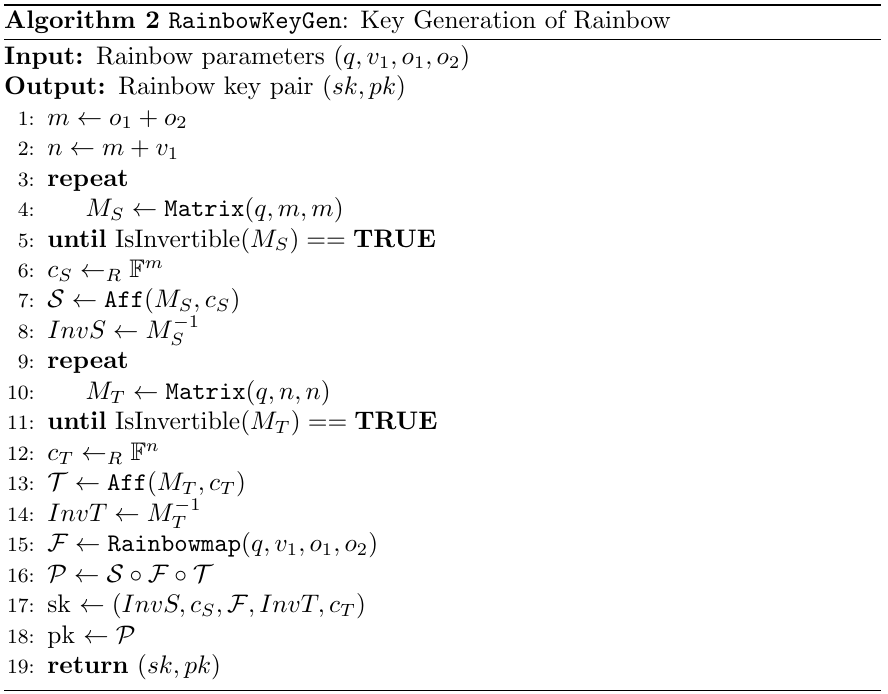
\includegraphics[width=\textwidth]{resources/rainbowkeygen.png}
    \caption{Pseudo code for the Rainbow key generation scheme.}
    \label{rainbowkeygen}
\end{figure}
As this sections has focus on the actual \texttt{c}-implementation of the reference Rainbow scheme, I will bridge the gap between this figure and what is found in the \texttt{Ia\_Classic\_Reference} folder.\medskip\\
Looking at \cref{rainbowkeygen} and making a coupling to \cref{rainscheme} one might clearly see the initialization of important aspects of the key, such as the affine invertible maps $S$ and $T$ generated as $M_S$ and $M_T$ respectively. This initialization is done in lines 3-14 in \cref{rainbowkeygen} whilst line 15 and onward is generation of the central map and at last the generation of the public and secret keys $pk$ and $sk$. The highest-level abstraction of this procedure lies in the \texttt{rainbow\_keypair.c} in \texttt{generate\_keypair()}. This functions is called from the \texttt{NIST}-specified \texttt{crypto\_sign\_keypair()} in \texttt{sign.c}. In \texttt{crypt\_sign\_keypair()} itself, before calling for the generation of a public-secret keypair, the \texttt{NIST} \texttt{randombytes()} function is called aswell ensuring that a securely generated seed of bytes is obtained. Once the keys have been generated, the memory of the seed is nullified.\medskip\\
Using the seed provided from the \texttt{randombytes()} function, \texttt{generate\_keypair()} then first calls \texttt{\_generate\_secretkey} which computes the $S$ and $T$ maps and returns. Once this has been done, the function goes on to compute the public key from the secret key just generated. This generation is first done by computing a temporary structure, namely \texttt{ext\_cpk\_t}, for the public key by computing the matrix $Q$ from the central map $F$. The matrix $Q$ can be seen in section 4.1 of \cite{rainbownist}. As was also stated in \cref{rainscheme} the public key is the composition of three maps such that the central map is obfuscated using $S$ and $T$. This obfuscations is primarily done by calling the \texttt{obfuscate\_l1\_polys()} function using various parts of the public key polynomials and secret key polynomials.
\medskip\\
The format of the generated public key is then a Macaulay matrix in column-major form, which has the monomials ordered in lexicographic order. Every two 4-bit coefficients are then packed into a single byte yielding no bit-waste for each coefficient \cite{rainbownist}. In an abstracted form, the public key is
$$
    [q_{1,1,1}, q_{1,1,2}, \dots,q_{1,1,m},q_{1,2,1} \dots , q_{1,n,m}, q_{2,2,1}, \dots q_{n,n,m}]
$$
where $q_{i,j,k}$ is the coefficient of monomial $x_ix_j$ in polynomial $p_k$.\medskip\\
As the nature of the private key requires a little more structure to index it by the different maps, it is stored with each map separately though in the order $S^{-1}$, $F$ and $T^{-1}$. In addition to the fact that the inverses of $S$ and $T$ are stored, $F$ is also deconstructed such that the two layers it is made up of are stored separately \cite{rainbownist}. The exact format of $S$ and $T$ can be seen in \cite{rainbownist}.
\subsubsection{Message Signing} \label{section:message_sign}
To sign a document with Rainbow, the scheme uses the inverted maps of $S$ and $T$ while computing a pre-image of some $\textbf{y} \in F$. The computations seen in \cref{rainbowsign} start, at a high abstractional layer, in the \texttt{NIST}-specified \texttt{crypto\_sign()} function in \texttt{sign.c}.\medskip\\
Before any computation involving aspects of the private key a message digest is created, using SHA256, of the input document/message. The hashing functionality used here is the one specified in \cref{utils} provided by \texttt{utils\_hash.c} wrapper file. Lines 2-4 in \cref{rainbowsign} is then computed using the \texttt{rainbow\_sign()} function provided by the \texttt{rainbow.c} file.
\begin{figure}[t]
    \centering
    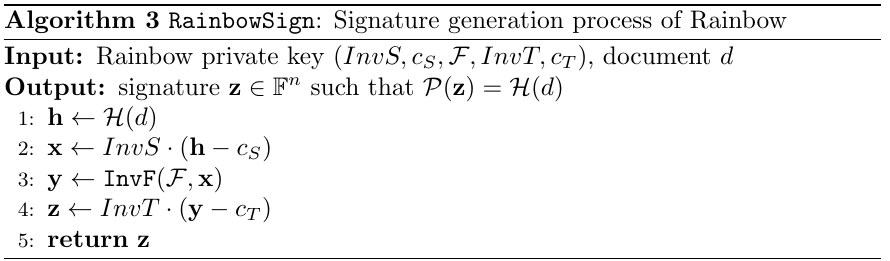
\includegraphics[width=\textwidth]{resources/rainbowsign.png}
    \caption{Pseudo code for the Rainbow signature scheme.}
    \label{rainbowsign}
\end{figure}\\
Due to the layered nature of the Rainbow scheme, the first part of \texttt{rainbow\_sign()} is used to randomly generate variables (called \emph{vinegar} variables), the linear equations of the first layer (using the \emph{vinegar} variables) while also pre-computing variables for the second \emph{rainbow layer}. Once this setup has been computed, the scheme is ready to compute line 2 in \cref{rainbowsign}.\medskip\\
As the scheme has to find a \emph{suitable} pre-image $\textbf{y} \in F$, it is not impossible to obtain a pre-image $\textbf{y}$ that is not suitable for further computation forcing the algorithm to find a new pre-image through a rerun. This is implemented as a \texttt{while}-loop running the computations of lines 2 and 3 until a point is reached where the result $\textbf{y}$ is \emph{suitable}. Such a $\textbf{y}$ would be one that allows for the system of linear equations, constructed by using the randomly generated \emph{vinegar} variables in the polynomials of $F$, to be solvable. Once the aforementioned system of linear equations is solvable $\textbf{y}$ is a suitable pre-image. The procedure can be seen in \cref{rainbowinvf}. Having computed lines 1-3 in \cref{rainbowsign}, the remaining part of the procedure is to use the pre-image $\textbf{y}$ to compute the signature $\textbf{z}$ and return that.
\begin{figure}[t]
    \centering
    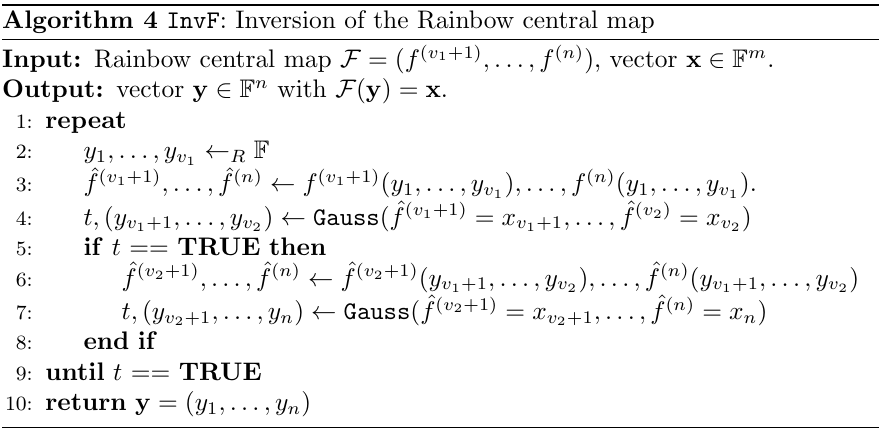
\includegraphics[width=\textwidth]{resources/rainbowinvf.png}
    \caption{Pseudo code inverting the central map $F$.}
    \label{rainbowinvf}
\end{figure}
To end off, the function \texttt{rainbow\_sign()} cleans the memory by nullifying all contents of the addresses used for the procedure.
\subsubsection{Signature Verification} \label{section:message_verif}
As the procedure in \cref{rainbowsign} uses pre-images and inverted maps to compute $\textbf{z}$, the verification procedure is quite simple. Provided a signature it can be verified by hashing the document/message in use, using the same hashing function as the signer did, and computing the public map on the given signature to then check if the values of both are the same. Figure \ref{rainbowveri} shows the pseudo code if this procedure. The procedure is, once more, ran from a \texttt{NIST}-specified function, though, this time called \texttt{crypto\_sign\_open()}. 
\begin{figure}[t]
    \centering
    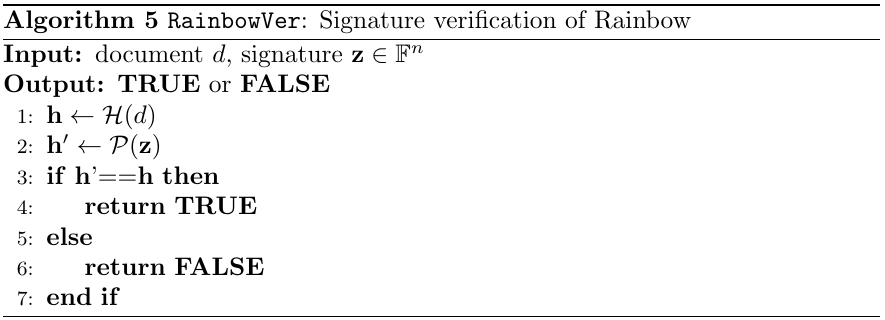
\includegraphics[width=\textwidth]{resources/rainbowver.png}
    \caption{Pseudo code for the Rainbow verification scheme.}
    \label{rainbowveri}
\end{figure}\\
For the sake of satisfactory computation, the same SHA scheme, namely SHA256, is used to compute the hash of the document $d$. Once more, the wrapper in \texttt{utils\_hash.c} is used to wrap the \texttt{RISCV-Crypto} implementation mentioned in \cref{utils}. To compute the publicmap on $\textbf{z}$, line 2 in \cref{rainbowveri}, the procedure calls \texttt{rainbow\_verify()} in \texttt{rainbow.c} to handle the remainder of the scheme.\medskip\\
The \texttt{rainbow\_verify()} function has two functionalities
\begin{enumerate}
    \item computing the publicmap using \texttt{rainbow\_publicmap()} in\\ \texttt{rainbow\_publicmap.c}, and
    \item verifying the computed publicmap against the hashed document value.
\end{enumerate}
The public map computation in \texttt{rainbow\_publicmap()} is much as one would expect for computing an output vector from a system of equations and some input the variables.\medskip\\
The actual verification is then done in \texttt{\_rainbow\_verify()} using the message digest computed by the \texttt{rainbow\_publicmap} procedure. The idea for verification checking is to check a locally hashed version of the document against the digest computed just prior. The check is a simple bit-wise \texttt{xor} for each \texttt{uint8\_t} (or just each byte) that resides in both hashes. For each byte value, the result of the bit-wise \texttt{xor} is then \texttt{or}'ed such that if the final value is larger than 0, the hashes are different and the verification returns a verification failure.

\subsubsection{Finite Field Arithmetic} \label{implementation:ffa}
%The mathematical aspect of the Rainbow scheme is quite large, as the core of the scheme is based on pure math. \textbf{NOT DONE}
As the polynomials in the public and private key maps are defined over finite fields much of the Rainbow scheme relies on finite field arithmetic, as well as aspects of linear algebra. Performing operations like message signing requires a gaussian elimination of a linear system, as was seen in \cref{section:message_sign}. For finite field arithmetic the code uses many finite field multiplications as well as finite field additions. These arithmetic operations are not native on all platforms, and therefore are implemented through the use of non-native algorithms.\medskip\\
The linear algebra and finite field arithmetic functions are implemented in the files \texttt{gf16.h}, all files prepended with \texttt{blas} and the \texttt{parallel\_matrix\_op} files (\texttt{.c} and \texttt{.h}). The original Rainbow code relies on using Single Instruction Multiple Data (SIMD) instructions on the benchmarked platforms to obtain fast computations in the specified finite fields, $GF(256)$ and $GF(16)$ that is.
\medskip\\
Specified in \cite{rainbownist}, the $GF(16)$ multiplications relies on using \texttt{VPSHUFB/TBL} instructions for multiplication tables. Using this approach, multiple $GF(16)$ elements can be multiplied by some $GF(16)$ scalar, using the aforementioned SIMD instructions. As these instructions are native to x86 and ARM platforms, the equivalent version for RISC-V is the vector instruction set extension. For this project, as was specified in \cref{pre-riscv}, the ISA used is RV32IM meaning that the vector instructions are not applied. This means that the potential difference in performance between the platforms tested in \cite{rainbownist} and this RISC-V platform potentially is quite different, as the compiler is no longer able to use SIMD instructions for these computations.
\medskip\\
An alternative implementation, for time-constancy, is also given by the Rainbow authors in \cite{rainbownist}. In this version, multiplications still rely on the SIMD instructions to obtain fast multiplications for multiple elements at a time. Though, instead of using multiplication tables the new multiplication method is using logarithm and exponentiation tables such that $a \cdot b = g^{(\log_g a +  \log_g b)}$ with $\log_g 0 = -42$ \cite{rainbownist}.
\medskip\\
The functions implementing the aforementioned functionality are used as subprocedures for the general public key evaluation method given by Tung Chou, as mentioned in \cite{rainbownist}. The specifics of this general method will not be gone through in this report. Intead, having focus on the finite field operations done by the Rainbow reference implementation, the functionality mentioned in the former paragraphs have been implemented in \texttt{blas\_u32.h}, \texttt{gf16.h} and \texttt{blas.h}. Specifically for Rainbow level I, the multiplication scheme used when evaluating the \texttt{GF(16)} coefficients of the multivariate polynomials against their corresponding monomials is done in \texttt{blas\_u32.h} using the \texttt{\_gf16v\_mul\_scalar\_u32()} function (being aliased \texttt{blas.h} to \texttt{gf16v\_mul\_scalar()}.
\medskip\\
Using Rainbow level III and V will require additional computations as the elements are over $GF(256)$ instead of $GF(16)$. These computations can either be done using the same SIMD instruction principles as was done for $GF(16)$ or using the Karatsuba algorithm to obtain a fast multiplication of elements. The latter of which uses the same representation as I did for the optimizations mentioned in \cref{opti}. Although these security levels were not in focus during this project, the reference functionality for them is still available such that any future optimization is easily available.
\subsection{Testing Environment}
As all aforementioned functionality was implemented and ran on a simulated device that does not interact with the host machine operating system in the same way that a typical program would, the testing facilities also had to be a little different. It therefore seems reasonable to shortly discuss how all aforementioned functionality was tested, as any errors in testing usually is quite a bad sign later in the pipeline. The primary file used for testing is the \texttt{kat.py} file in the \texttt{test/} directory.\medskip\\
First of all, to be able to test the scheme the host device and the client device had to be able to communicate. Usually this can be done via some sort of serial port on an actual device, though as this was a virtual device a serial port was not present. The author(s) of the \texttt{pqriscv} project ensured there to be a runtime option that allows for the client device to have a communications port through a linux \texttt{pts} device.\medskip\\
Before any actual communication between client and \texttt{kat.py}, the \texttt{kat.py} script will run some preparations to ensure that it is ready to check for correct outputs from the client device. For \texttt{kat.py} to check correctness it has access to a host-native Rainbow implementation, directly pulled from the github submission repository, which it then compiles and runs before any testing on the client device. This means that before any test, the \texttt{kat.py} file will generate a \texttt{KAT\_<timestamp>} folder that holds the randomseed used, the keys generated from the random seed, the message, an incorrect signature (although this is generated, it is not of importance for the current state of the test-suite) and the signature generated given the keys and message in the folder. This collection of files constitutes a \textit{Known Answer Test} or KAT and is used by the \texttt{kat.py} script to check for correctness in the implementation.\medskip\\
The initial communication between the test-suite and the client device has the test-suite send all required items to the client device. When key-generation is tested, the input is just the random seed needed for the client device to generate a keypair. For signing and verification the test-script will send the message, a key (public for verification and private for signing) and a signature, being of course only for verification. Once these values have been provided, the script will wait for the client device to answer. For key generation the script checks if the byte-values of the host-native scheme are equal to the byte values of the client scheme. For signing, only signature byte-values are checked, while verification checks for any inconsistencies in the \texttt{true}/\texttt{false} output of the client, still compared to the host-native version.
\medskip\\
The testing script is also accompanied by a shell-script, called \texttt{multitest.sh}, for running multiple tests or benchmarks on the different implementations and saving the results in the corresponding \texttt{KAT} folder. Using the output of potential benchmark runs (after running \texttt{multitest.sh}), the \texttt{grapher.py} script allows for easy bar-plotting of key aspects for evaluation.
        \section{Optimizations} \label{opti}
For this project multiple approaches were tested for running Rainbow on a constrained-computing platform such as those typically seen in embedded devices. Section \ref{opt:gf16comp} goes into detail on how elements of GF16 are treated for the optimizations of this project. It also specifies the notation used in \cref{opt:lookup} and \cref{opt:bitslice}. The latter two sections each show how the theoretical aspect of the optimization works as well as showing how it was implemented.
\subsection{GF(16) Computation} \label{opt:gf16comp}
The subsequent sections after this, the notation assumes a bit of knowledge on how a $GF(16)$ element can be represented. Any element in $GF(16)$ can be represented as a \emph{polynomial of polynomials}. What is meant by this is that any element in $GF(16)$ can take the form
$$
    \alpha b + \beta
$$
where $\alpha$ and $\beta$ both are of the form 
$$
    \gamma a + \delta
$$
such that the \emph{outermost} polynomial is linear over variable $b$ and the two \emph{innermost} are linear over the variable $a$. This is the same as expressing a $GF(16)$ element as a first-degree polynomial with first degree polynomials as coefficients. Representing a $GF(16)$ value this way is also called \emph{Tower-field representation}.
\medskip\\
Using Tower-field representation for $GF(16)$ elements has the coefficients of the \emph{outermost} degree-1 polynomial be $GF(4)$ elements, which themselves are represented as the degree-1 polynomials over the variable $b$. The coefficients of the \emph{innermost} polynomial would then be $GF(2)$ elements, holding exactly a binary value.
\medskip\\
By the above constructions it is then clear that a $GF(16)$ value can be represented using two, layered, polynomials where the innermost has binary coefficients, also called Tower-field representation. An example of such a $GF(16)$ coefficient could be
$$
    (1a + 0) b + (1a + 1)
$$
Further, for the following subsections I expand upon this by writing such a polynomial either as the bitstring (using the above element as reference)
$$
    1011
$$
or using square brackets to denote the coefficients of the innermost polynomial
$$
    [10]b + [11] = [10][11].
$$
\subsection{Lookup Tables} \label{opt:lookup}
For a system over $GF(16)$ coefficients, the elements might take one of 16 different values. Throughout the publicmap computation, multiplication over such $GF(16)$ values are done quite a few times. However, most modern architectures, and especially the \texttt{RISC-V} architecture, have not been built to support arithmetic over such finite fields. For this reason, to test whether or not the bit-manipulation approach in the reference code is a bottleneck, I used a basic lookuptable approach to compute the multiplication result of two values in $GF(16)$.\medskip\\
Computing the $16 \times 16$ table of $GF(16)$ elements was done using the original multiplication code and running it for each combination of $GF(16)$ values that exist. 
The table looks as \cref{lookuptable} and lies in the \texttt{gf16.h} file, in the function \texttt{gf16\_mul()}.
\begin{figure}[t]
    \centering
    \begin{tabular}{|c|c|c|c|c|c|c|}
        \hline
            \textbf{Polynomials} & \textbf{0000} & \textbf{0001} & \textbf{0010} & \textbf{0011} & \dots & \textbf{1111} \\
        \hline
            \textbf{0000} & 0000 & 0000 & 0000 & 0000 & \dots & 0000\\
        \hline
            \textbf{0001} & 0000 & 0001 & 0010 & 0011 & \dots & 1111\\
        \hline
            \vdots & \vdots & \vdots & \vdots & \vdots & $\ddots$ & \vdots\\
        \hline
            \textbf{1111} & 0000 & 1111 & 0101 & 1010 & \dots & 1001\\
        \hline
    \end{tabular}
    \caption{A brief view at some of the lookuptable elements}
    \label{lookuptable}
\end{figure}\\
Since each $GF(16)$ can be stored in one \texttt{uint8\_t} each, it is possible to have at most 256 (plus, potentially some overhead bytes) bytes of space used for a table like above. Given a constrained system like this, a space-speed tradeoff have to be considered thoroughly. This tradeoff will be evaluated further in \cref{evalsec}.\medskip\\
The specific implementation uses two $GF(16)$ elements, $a$ and $b$, as input and indexes the table using $a*16 + b$, as both $a$ and $b$ are promised to maximally use four bits of memory. This, of course, needs some external checks on the amount of bits used in $a$ and $b$ to be fully secure, though it was not seen as a major insecurity on the system to be addressed immediately.
\medskip\\
Should it be a problem using \texttt{256} bytes of memory, some memory can be saved by not computing multiplications where one polynomial is of value $0$ or $0001$s but just returning a $0$ byte to the caller, in case of $0$. When one of the polynomials is of value $0001$ the case is equally as trivial, where the procedure should just return the other polynomial. The tradeoff here is then that the indexing of the table might become a bit more intricate than it is now plus an additional check is required before any actual lookup is done.
\medskip\\
Further, when the code calls \texttt{gf16v\_mul\_scalar()}, it goes through all the $GF(16)$ elements provided in the \texttt{uint8\_t *a} array, multiplying the value of \texttt{uint8\_t gf16\_b} onto each. Due to the nature of the public map computation, the calls to this multiplication function happens quite a few times with various sizes of the array \texttt{a}. This implies that going through each element of \texttt{a} one-by-one might have some performance implications as well. This will be evaluated in \cref{evalsec}.
\subsection{Bitslicing} \label{opt:bitslice}
This subsection seeks to show how bitslicing for this project was tackled on both a more theoretical level aswell as how it was implemented in reality. For \cref{bitslice:theory} the theoretical design of the system is discussed, while \cref{bitslice:implementation} provides and explanation of how it was brought to actual \texttt{c}-code.
\subsubsection{Design of a Bitsliced System for GF(16)} \label{bitslice:theory}
To start this section off, the basic approach to multiplying two polynomials with polynomial coefficients is shown. Such a polynomial has the form
$$
    f = f_1b + f_0,
$$
where all
$$
    f_i = f_{i1}a+f_{i0}
$$
are the \emph{inner} polynomials of $f$ for $i = 0$ and $i = 1$ such that $f_1, f_0 \in GF(4)$ and $f_i1, f_i0 \in GF(2)$\\ 
Given any two such polynomials,
\begin{equation*}
    \begin{split}
        f &= (f_{11}a+f_{10})b + (f_{01}a + f_{00})\\
        g &= (g_{11}a+g_{10})b + (g_{01}a + g_{00})
    \end{split}
\end{equation*}
the product can be computed by
\begin{equation} \label{bitslice:poly}
    \begin{split}
        f \cdot g &= (f_{11}a + f_{10})(g_{11}a + g_{10})b^2\\
        &+ (f_{11} a + f_{10})(g_{01}a + g_{00})b\\ 
        &+ (f_{01}a + f_{00})(g_{11}a + g_{10})b\\ 
        &+ (f_{01} a + f_{00})(g_{01}a + g_{00})\\
        &= (f_{11}g_{11}a^2 + (f_{11}g_{10} + f_{10}g_{11})a + f_{10}g_{10})b^2\\
        &+ (f_{11}g_{01}a^2 + (f_{11}g_{00} + f_{10}g_{01})a + f_{10}g_{00})b\\
        &+ (f_{01}g_{11}a^2 + (f_{01}g_{10} + f_{00}g_{11})a + f_{00}g_{10})b\\
        &+ (f_{01}g_{01}a^2 + (f_{01}g_{00} + f_{00}g_{01})a + f_{00}g_{00})\\
    \end{split}
\end{equation}
Using the above notions we are able to construct a theoretical plan for bitslicing.
\medskip\\
Now, provided some MQ system over $GF(16)$ with $64$ polynomials in total, as this project has Rainbow level $I$ in focus, the \emph{Tower-field representation} mentioned in \cref{opt:gf16comp} is suitable. Given this representation, it is possible to decompose any multiplication and addition operation over two $GF(16)$ elements into a simple $\xor$ or $\wedge$ operation, respectively. In \cref{opt:gf16comp} it was discussed that this representation of $GF(16)$ elements decomposes into \emph{layered} polynomials of $GF(2)$ elements. As elements of $GF(2)$ is a binary number system, the two formerly mentioned operations are well-defined and certainly part of typical ISAs as \texttt{xor} and \texttt{and} instructions.\medskip\\
For the two $GF(16)$ values in Tower-field representation
$$
    x = [11]b + [01]
$$
and
$$
    y = [01]b + [01]
$$
the product is computed by
\begin{equation*}
    \begin{split}
        x \cdot y &= ((1a + 1)b + (0b + 1)) \cdot ((0a + 1)b + (0a + 1))\\
        &= ((1 \wedge 0)a^2 + ((1 \wedge 1) \xor (1 \wedge 0))a + (1 \wedge 1))b^2\\ 
        &+ ((1 \wedge 0)a^2 + ((1 \wedge 1) \xor (1 \wedge 0))a + (1 \wedge 1))b\\
        &+ ((0 \wedge 0)a^2 + ((0 \wedge 1) \xor (1 \wedge 0))a + (1 \wedge 1))b\\
        &+ ((0 \wedge 0)a^2 + ((0 \wedge 1) \xor (1 \wedge 0))a + (1 \wedge 1))\\
        &= (0a^2 + 1a + 1)b^2 + (0a^2 + 1a + 1)b + (0a^2 + 0a + 1)b\\
        &+ (0a^2 + 0a + 1)\\
    \end{split}
\end{equation*}
where any $+$ not converted to an $\xor$ resembles a plus operation \emph{kept intact} with the purpose of keeping the polynomial structure of the element. Rephrased, these plusses resemble the borders of the different degrees of the three terms. Further developing the above computation for $GF(16)$ specifically would require the two linear terms to be term-wise/bit-wise \texttt{xor}'ed providing a single linear term.
\begin{equation*}
    \begin{split}
        x\cdot y &= (0a^2 + 1a + 1)b^2 + ((0 \xor 0)a^2 + (1 \xor 0)a + (1 \xor 1))b + (0a^2 + 0a + 1)\\
        &= (a + 1)b^2 + (a + 0)b + (0a + 1)
    \end{split}
\end{equation*}
As multiplying two first degree polynomials, with linear terms having nonzero coefficients, results in a quadratic term, the polynomial above has to be \emph{reduced} for it to comply with the Tower-field representation and for it to only represent a $GF(16)$ value. A reduction like this is done by \texttt{xor}'ing the quadratic term (the bits of $q$ in $qb^2$) multiplied by $1$ onto the linear term and by $a$ onto the constant term. This is also what is called a \emph{reduction polynomial} which in this case takes the form of $b^2 + b + a$. Many alternatives, like $b^2 + b + 1$, exist, though the aforementioned one was chosen by the Rainbow authors. Using this, the reduction of the $GF(16)$ element is
\begin{equation*}
    \begin{split}
        x\cdot y &= ((a + 0) + (a + 1)*(0a + 1))b + ((0a + 1) + (a + 1)*(a + 0))\\
        &= ((a + 0) + (a + 1))b + ((0a^2 + 0a + 1) + (a^2 + a + 0)))\\
        &= ((a + 0) + (a + 1))b + ((0a^2 + 0a + 1) + ((1 \xor 1)a + (1 \xor 0)))\\
        &= ((a + 0) + (a + 1))b + ((0a + 1) + (0a + 1))\\
        &= ((1 \xor 1)a + (0 \xor 1))b + ((0 \xor 0)a + (1 \xor 1))\\
        &= (0a + 1)b + (0a + 0).
    \end{split}
\end{equation*}
The reduction of the $GF(4)$ values, or the \textit{inner} polynomials, were done by \texttt{xor}'ing the quadratic term onto the linear and constant terms respectively (which was not necessary in this example as all quadratic terms were 0). This means that a different \emph{reduction polynomial} was used for $GF(4)$, namely $a^2 + a + 1$. Formally, we have
$$
    GF(4) = GF(2)[a]/(a^2 + a + 1)
$$
and
$$
    GF(16) = GF(4)[b]/(b^2 + b + a).
$$
To be able to provide a potential speedup for Rainbow, all operations are going to be on multiple elements at once. This means that any multiplication performed on a term of the public key $P$ and corresponding values of the signature $\textbf{z}$ will be computed using multiple terms of the public key at once. To help with this, denote four \emph{registers} for holding certain bits of a $GF(16)$ elements for this theoretical bitslicing construction.
\begin{enumerate}
    \item $r_3$ holding the high order bits of the "high-order polynomials",
    \item $r_2$ holding the low-order bits of the "high-order polynomials",
    \item $r_1$ holding the high-order bits of the "low-order polynomials" and
    \item $r_0$ holding the low-order bits of the "low-order polynomials".
\end{enumerate}
The usage of these can be shown by providing the toy system $P$ (though, this system is not compliant with any of the security levels of Rainbow):
\begin{equation*}
    \begin{split}
        p_1(x,y) &= ([01]b + [11]) xy + ([11]b + [00]) x + ([10]b + [01]) y + ([11]b + [11])\\
        p_2(x,y) &= ([00]b + [11]) xy + ([01]b + [01]) x + ([10]b + [10]) y + ([10]b + [01])\\
        p_3(x,y) &= ([00]b + [00]) xy + ([10]b + [00]) x + ([01]b + [10]) y + ([10]b + [11])
    \end{split}
\end{equation*}
For the $xy$ term, across polynomials of $P$, the computation uses the \emph{register}-values (visually shown as column vectors):
$$
    r_3 = \begin{bmatrix} 0\\ 0\\ 0 \end{bmatrix}, r_2 = \begin{bmatrix} 1\\ 0\\ 0 \end{bmatrix}, r_1 = \begin{bmatrix} 1\\ 1\\ 0 \end{bmatrix}, r_0 = \begin{bmatrix} 1\\ 1\\ 0 \end{bmatrix}.
$$
Then, any \emph{index} of $\textbf{z}$ can be expanded to a corresponding set of vectors. That is, using indices of \textbf{z} we obtain the value of the \emph{monomial} of the current term in the $MQ$ system. The value of $xy$, computed earlier, will now be used as the current monomial to showcase the computation upon an entire system. This kind of procedure uses an accumulator that in the end is the final result of the computation. That is, let $total$ be a vector of size three for this example (size $m$ in general). When the computation is done
$$
    total = P(\textbf{z}).
$$
Initially we have:
$$
    total = 
    [
    \begin{bmatrix}
        0\\
        0\\
        0
    \end{bmatrix}a
    + 
    \begin{bmatrix}
        0\\
        0\\
        0
    \end{bmatrix} ]
    [
    \begin{bmatrix}
        0\\
        0\\
        0
    \end{bmatrix}a
    + 
    \begin{bmatrix}
        0\\
        0\\
        0
    \end{bmatrix} 
    ] = \begin{bmatrix}
        [00][00]\\
        [00][00]\\
        [00][00]
    \end{bmatrix}.
$$
Provided the value $xy = [01][00]$, we can expand $xy$ such that each \textit{bit} becomes a vector in $\mathbb{R}^m$ consisting of all $1$s or all $0$s. For this value of $xy$ the corresponding \textit{expanded} values are:
$$
    \textbf{xy} = 
    [
    \begin{bmatrix}
        0\\
        0\\
        0
    \end{bmatrix}a
    + 
    \begin{bmatrix}
        1\\
        1\\
        1
    \end{bmatrix} ]
    [
    \begin{bmatrix}
        0\\
        0\\
        0
    \end{bmatrix}a
    + 
    \begin{bmatrix}
        0\\
        0\\
        0
    \end{bmatrix} 
    ] = \begin{bmatrix}
        [01][00]\\
        [01][00]\\
        [01][00]
    \end{bmatrix}.
$$
Once more we use the structure of the latter equality of \cref{bitslice:poly} as a template for structure the computation. Letting the coefficients of $\textbf{xy}$ be named $\textbf{xy}_3$, $\textbf{xy}_2$, $\textbf{xy}_1$, $\textbf{xy}_0$ such that:
$$
    \textbf{xy}_3 = \begin{bmatrix} 0\\ 0\\ 0 \end{bmatrix}, \textbf{xy}_2 = \begin{bmatrix} 1\\ 1\\ 1 \end{bmatrix}, \textbf{xy}_1 = \begin{bmatrix} 0\\ 0\\ 0 \end{bmatrix}, \textbf{xy}_0 = \begin{bmatrix} 0\\ 0\\ 0 \end{bmatrix},
$$
we can model the computation for the first term of the $MQ$ polynomials as:
\begin{equation*}
    \begin{split}
        t_2 &= ((r_3 \wedge \textbf{xy}_3)a^2 + ((r_3 \wedge \textbf{xy}_2) \xor (r_2 \wedge \textbf{xy}_3))a + (r_2 \wedge \textbf{xy}_2))b^2,\\
        t_{10} &= ((r_3 \wedge \textbf{xy}_1)a^2 + ((r_3 \wedge \textbf{xy}_0) \xor (r_2 \wedge \textbf{xy}_1))a + (r_2 \wedge \textbf{xy}_0))b,\\
        t_{11} &= ((r_1 \wedge \textbf{xy}_3)a^2 + ((r_1 \wedge \textbf{xy}_2) \xor (r_0 \wedge \textbf{xy}_3))a + (r_0 \wedge \textbf{xy}_2))b,\\
        t_0 &= ((r_1 \wedge \textbf{xy}_1)a^2 + ((r_1 \wedge \textbf{xy}_0) \xor (r_0 \wedge \textbf{xy}_1))a + (r_0 \wedge \textbf{xy}_0)),
    \end{split}
\end{equation*}
where each of these temporary \textit{inner} polymials represent a term of the \textit{outer} polynomial. The logic-operations of \texttt{xor} and \texttt{and} is then done index-wise across column vectors and term-wise across polynomials. An example is the computation of $t_1 = t_{10} \xor t_{11}$ where the computations are done like so:
\begin{equation*}
    \begin{split}
        t_{10} &= ((\begin{bmatrix} 0\\ 0\\ 0 \end{bmatrix} \wedge \begin{bmatrix} 0\\ 0\\ 0 \end{bmatrix})a^2 + ((\begin{bmatrix} 0\\ 0\\ 0 \end{bmatrix} \wedge \begin{bmatrix} 0\\ 0\\ 0 \end{bmatrix}) \xor (\begin{bmatrix} 1\\ 0\\ 0 \end{bmatrix} \wedge \begin{bmatrix} 0\\ 0\\ 0 \end{bmatrix}))a + (\begin{bmatrix} 1\\ 0\\ 0 \end{bmatrix} \wedge \begin{bmatrix} 0\\ 0\\ 0 \end{bmatrix}))b,\\
        t_{10} &= (\begin{bmatrix} 0\\ 0\\ 0 \end{bmatrix}a^2 + \begin{bmatrix} 0\\ 0\\ 0 \end{bmatrix}a + \begin{bmatrix} 0\\ 0\\ 0 \end{bmatrix})b,\\
        t_{11} &= ((\begin{bmatrix} 1\\ 1\\ 0 \end{bmatrix} \wedge \begin{bmatrix} 0\\ 0\\ 0 \end{bmatrix})a^2 + ((\begin{bmatrix} 1\\ 1\\ 0 \end{bmatrix} \wedge \begin{bmatrix} 1\\ 1\\ 1 \end{bmatrix}) \xor (\begin{bmatrix} 1\\ 1\\ 0 \end{bmatrix} \wedge \begin{bmatrix} 0\\ 0\\ 0 \end{bmatrix}))a + (\begin{bmatrix} 1\\ 1\\ 0 \end{bmatrix} \wedge \begin{bmatrix} 1\\ 1\\ 1 \end{bmatrix}))b,\\
        t_{11} &= (\begin{bmatrix} 0\\ 0\\ 0 \end{bmatrix}a^2 + \begin{bmatrix} 1\\ 1\\ 0 \end{bmatrix}a + \begin{bmatrix} 1\\ 1\\ 0 \end{bmatrix})b,\\
        t_1 &= ((\begin{bmatrix} 0\\ 0\\ 0 \end{bmatrix} \xor \begin{bmatrix} 0\\ 0\\ 0 \end{bmatrix})a^2 + (\begin{bmatrix} 0\\ 0\\ 0 \end{bmatrix} \xor \begin{bmatrix} 1\\ 1\\ 0 \end{bmatrix})a + (\begin{bmatrix} 0\\ 0\\ 0 \end{bmatrix} \xor \begin{bmatrix} 1\\ 1\\ 0 \end{bmatrix}))b,\\
        t_1 &= (\begin{bmatrix} 0\\ 0\\ 0 \end{bmatrix}a^2 + \begin{bmatrix} 1\\ 1\\ 0 \end{bmatrix}a + \begin{bmatrix} 1\\ 1\\ 0 \end{bmatrix})b.
    \end{split}
\end{equation*}
Once the temporary values have been computed, they potentially need to be reduced to remove any quadratic term. The first reduction done is on the $GF(4)$ elements, namely the polynomials over $a$. This is done, as specified earlier, by \texttt{xor}'ing (this time index-wise in each vector/register) the $a^2$ term onto the other two terms. Following the reduction of the $GF(4)$ elements, a reduction of the $GF16$ element as a whole can be reduced. To do this, the temporary value $t_2$ is multiplied by:
$$
    \begin{bmatrix}
        1\\
        1\\
        1
    \end{bmatrix}a 
    + 
    \begin{bmatrix}
        0\\
        0\\
        0
    \end{bmatrix}
$$
in the same fashion as when multiplying $\textbf{xy}$ with the coefficients held in the registers $r_i$, $i = 1,\dots, 4$. The result of this multiplication is then \texttt{xor}'ed onto $t_0$ term-wise. For $t_1$ the value of $t_2$ itself is \texttt{xor}'ed onto (no multiplication needed).\medskip\\
Once the results of reducing $GF(16)$ element (the \textit{outer} polynomial) has been done, the values of $t_1$ and $t_0$ are \texttt{xor}'ed term-wise onto \textit{total}:
$$
    total = [[00] \xor t_1] [[00] \xor t_0].
$$
This way, \textit{total} accumulates the results of doing term-wise $GF(16)$ multiplications by summing the products, as well as doing it on all $m$ coefficients of the current term (across polynomials).
\subsubsection{Implementation of the Bitsliced Scheme} \label{bitslice:implementation}
To provide the functionality described in \cref{bitslice:theory}, three extra files were added to the implementation. These files are \texttt{slice.c}, \texttt{sliced\_arithmetic.c} and \texttt{slice.h}. An extra file is also added to the implementation which allows for easier transitioning between the three implementations (lookup tables, bitsliced and standard) through c preprocessor definitions. This file is called \texttt{impl.h} and chooses an implementation based on either it being empty or having one of the two preprocessor definitions commented out.
\medskip\\
The implementation of a bitsliced Rainbow scheme is done entirely through \texttt{c}-code, as one might have guessed from the files just mentioned, with no inline assembly or alike. Doing this allowed for abstracting many of the complex areas and operations of implementing bitsliced machinery. Using some, or purely, assembly code might have given an edge on performance, however, as the scope of this project is limited a purely assembly version was deemed too demanding.
\paragraph{GF(16) representation}
$GF(16)$ elements, represented with tower-field representation, are composed of two \texttt{c} \texttt{struct}s. The \texttt{struct}s used for this representation takes quite heavy inspiration from the graphical way the bitsliced scheme was represented in \cref{bitslice:theory} using vectors. The \texttt{struct}s used are divide into two groups: 1) \emph{high-level polynomials}, and 2) \emph{low-level polynomials}. These high- and low-level polynomials should not be mistaken with the actual polynomials of an $MQ$ system, though, instead should be seen as the \emph{outer}- and \emph{inner}-polynomials mentioned in \cref{bitslice:theory}. The actual \texttt{struct}s given in \texttt{slice.h} are \texttt{hl\_poly} and \texttt{ll\_poly}.
\medskip\\
A high-level polynomial, also an \emph{outer}-polynomial, would be a structure holding all four register values $r_0$, $r_1$, $r_2$ and $r_3$, or similar values like $\textbf{xy}$ from \cref{bitslice:theory}. For Rainbow level I, there are $64$ polynomials in total, meaning that one slice should be able to hold 64 different $GF(16)$ values where their individual bits are being distributed across these four vectors.
\medskip\\
To work with four vectors of length $64$, an \texttt{ll\_poly} \texttt{struct} is created. This creates a container for two vectors, either the two \emph{high-order} vectors or the two \emph{low-order} vectors. The $64$-dimensional vectors are then stored as \texttt{uint32\_t} arrays of length 2, in the members \texttt{snd}, \texttt{fst} and \texttt{cnst}. As can be deduced from the naming schemes, this \texttt{struct} allows for a potential \emph{quadratic} term, easing some complexities. In opposition to the \texttt{ll\_poly} being able to hold a \emph{quadratic} term, the \texttt{hl\_poly} does not allow for a \texttt{quadratic} term, but instead only holds the members \texttt{high} and \texttt{low} representing the high- and low-order bits or, alternatively, the linear and constant terms of the \textit{outer}-polynomials.
\paragraph{Obtaining GF(16) elements}
Slicing a column of 64 terms in the Macaulay matrix to a corresponding \texttt{hl\_poly} is built to work with the public key storage method, mentioned in \cref{section:keygen}, that the original authors of Rainbow provided. Now, denote the bits that would have gone into register $r_i$ (in \cref{bitslice:theory}) as $r_i$-bits. Using the \texttt{slice\_column()} function defined in \texttt{slice.c}, a column is stored with the $r_3$- and $r_2$-bits in the \texttt{hl\_poly.high} member, with \texttt{hl\_poly.high} being an \texttt{ll\_poly}. These bits are specifically stored in the \texttt{hl\_poly.high.fst} and \texttt{hl\_poly.high.cnst} arrays, for $r_3$- and $r_2$-bits respectively. The case for the $r_0$- and $r_1$-bits is symmetric, using the \texttt{hl\_poly.low} member instead.
\paragraph{Arithmetic operations} Once a column has been sliced, various operations take place on the sliced column and the corresponding $x_i$ and $x_j$ values given for this term of the $MQ$ system. These operations are primarily multiplications and additions on $GF(16)$ elements. However, as seen in \cref{bitslice:theory}, these operations rely on corresponding $GF(4)$ and $GF(2)$ versions. As $GF(2)$ elements act like simple binary values, without carries, the operations are \texttt{xor} and \texttt{and}. 
\medskip\\
For the \emph{inner}-polynomials, the operations of addition, multiplication and reduction are implemented in the functions \texttt{gf4\_nonpure\_add()}, \texttt{gf4\_prod()} and \texttt{gf4\_reduce()}. To be able to work with non-reduced, thereby \emph{nonpure}, \emph{inner}-polynomials the addition operation is allowed to add together quadratic terms of two, in advance, \emph{nonpure} $GF(4)$ polynomials. The reasoning behind this is mostly to save a few computations when computing the $t_1$ term of the \emph{outer}-polynomial as only one reduction is then needed in the aftermath (this computation was shown in \cref{bitslice:theory}).
\medskip\\
In contrast to the assumptions made by the addition functionality, a multiplication of two such \emph{inner}-polynomials is done assuming that their quadratic terms are zero. This assumption is important, as any value in such a quadratic term is forgotten and only the linear and constant terms are used for the multiplication. This also means that the output \texttt{ll\_poly} of the function is a \emph{nonpure}. The operation itself is mostly as was showcased in the toy-system of \cref{bitslice:theory}, of course being altered with regard to how the 64-dimensional vectors are stored in actuality.
\medskip\\
Once a sum or product of two of these bitsliced representation of $GF(4)$ values have been obtained, a reduction is potentially needed. The functionality itself is implemented in \texttt{gf4\_reduce()}. This function yields the $GF(4)$ reduction by doing an bit-wise \texttt{xor} on the elements of the \texttt{uint32\_t} arrays constructing the bitsliced $GF(4)$ element. That is, the operation is simply using the \texttt{xor} operator in \texttt{c} to do bit-wise \texttt{xor}'ing on the members of the input \texttt{ll\_poly}.
\medskip\\
To provide the arithmetic operations required for bitsliced $GF(16)$ elements, the operations are divided into a \emph{divide and conquer}-esque approach. The addition operation is the simplest, as it simply adds together the internal \texttt{ll\_poly}s using \texttt{gf4\_nonpure\_add()}. This addition is done by adding the \emph{high}-order bits and the low-order bits, respectively. For this process it is assumed that the internal \texttt{ll\_poly}s are \emph{pure}, such that their member \texttt{uint32\_t *snd} is all zeros.
\medskip\\
For multiplication of bitsliced $GF(16)$ elements, the code has to take a few more steps than the simpler addition process. As can be seen in the examples in \cref{bitslice:theory}, multiplying two of these \emph{outer}-polynomials, or bitsliced $GF(16)$ elements, requires multiplying their linear terms together (linear terms over $b$ if relating to the structure used in \cref{bitslice:theory}), their constant terms, and a combination of linear and constant terms. All of this is done using the $gf4\_*$ procedures given earlier, using the \emph{high}- and \emph{low}-order polynomials (or bits, depending on perspective) of the two \emph{outer}-polynomials of the bitsliced $GF(16)$ values. The computation itself follows mostly what was seen in the examples in \cref{bitslice:theory}, though now using the structures and functions just described. Reducing the \emph{outer}-polynomial with the correct \emph{reduction polynomial} is done by also computing a temporary \texttt{hl\_poly} resembling the $(1a+0)$ that is multiplied onto $t_2$ in \cref{bitslice:theory}.
\paragraph{Remainder of the bitslicing system}
Some functions in the three bitslicing-related files are purely helper functions, required for easily abstracting away the process of constructing a \texttt{hl\_poly} from two \texttt{ll\_poly}s and constructing an \texttt{ll\_poly} from three \texttt{uint32\_t} arrays (quadratic, linear and constant term).
\medskip\\
The more interesting aspects of this bitslicing implementation is how the public key, Macaulay matrix, is \emph{sliced} such that 64 coefficients are held in one \texttt{hl\_poly} (and how it goes back), how the system actually computes $P(\textbf{z})$ and how it obtains the bitsliced \emph{expansion} of the monomial for the current term. As the process of obtaining bitsliced values was already gone through, the remainder of this section focuses on the other functionality just listed.
\medskip\\
Computing $P(\textbf{z})$ using bitslicing was done by going through all columns of the Macaulay matrix that the public key consist of. Using the procedure given earlier, a column is sliced by using the \texttt{slice\_column()} function, which internally calls \texttt{slice\_32()} (twice), which slices 32 consecutive public key values (given the \emph{packed} format mentioned in \cref{section:keygen}). Once an \texttt{hl\_poly} representing 64 sliced coefficients of the $MQ$ system has been constructed, the code obtains the correct $x_i$ and $x_j$ from the signature by using the same indexing as the public key does. Obtaining these values from the signature \textbf{z} then yields two \texttt{uin8\_t} values that are expanded, like $xy$ was in \cref{bitslice:theory}, and then computing the product of the two along with $x_ix_j \cdot q_{i,j}$ ($q_{i,j}$ being the sliced $GF(16)$ values of this column). These are then accumulated, by addition, in an \texttt{hl\_poly} called \texttt{total}. This procedure is implemented in \texttt{sliced\_compute\_publicmap()} in \texttt{slice.c}.
\medskip\\
Expanding a single $GF(16)$ value to an \texttt{hl\_poly} is a simple operation that just checks the four lowest bits of the \texttt{uint8\_t} value and fills the entire corresponding \emph{vector} (symmetrically, the \texttt{uin32\_t} arrays used in \texttt{c}-code) with either 1s or 0s depending on the value of the specific bit.
\medskip\\
Once the system is done computing $P(\textbf{z})$ the \texttt{uint8\_t} values (also, individual $GF(16)$ elements) of the resulting message digest are stored in \texttt{total}. To convert this to a more readable, and more intuitive, format the implementation uses the \texttt{deslice()} function from \texttt{slice.c} to \emph{deslice} \texttt{total} into an array of 64 \texttt{uint8\_t} values. Obtaining this array is done by looking at the same bit-index in all four 64-dimensional vectors (using this analogy for clarity) and constructing a \texttt{uint8\_t} from the four resulting bits. Once an array of 64 \texttt{uint8\_t} ($GF(16)$) elements is constructed, these are packed similarly to how the public key was packed such that two $GF(16)$ elements are placed in a byte, resulting in a \texttt{uint8\_t} array of size 32. This last part is to stay consistent with how the Rainbow reference code stores the digest.
        \section{Evaluation} \label{evalsec}
Optimizing code to use special techniques does not ensure that the final code will run faster than the original code. For this reason, the following section will look into what is gained and what is lost by each optimization type. The primary evaluation will be on CPU cycles and cycle/instruction ratio, as timed benchmarks would possibly yield unreliable results., due to overhead between the communicating parties (especially the possible overhead of the extra computation done by the test environment). Asking for cycles and instruction used on the \texttt{PQ-VexRiscV} CPU is easily done using a Hardware Abstraction Layer that exposes a \texttt{c} API with exactly this functionality (plus some).
\begin{figure}[t]
    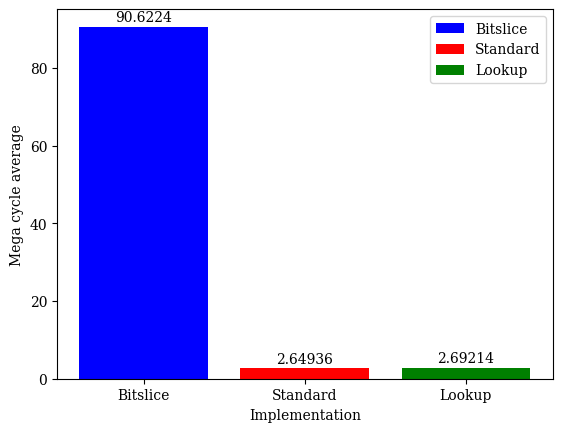
\includegraphics[width=0.5\textwidth]{resources/bar_avg_cycle.png}
    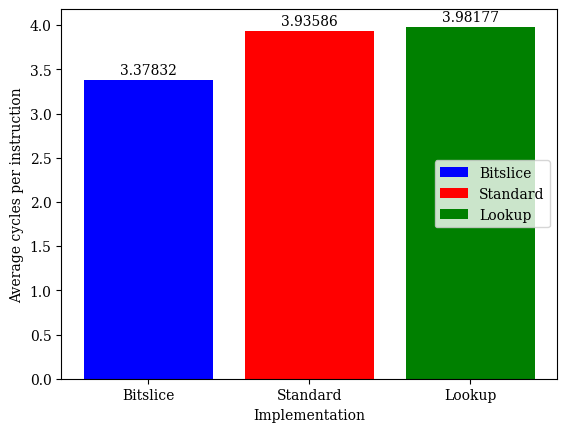
\includegraphics[width=0.5\textwidth]{resources/bar_avg_ratio.png}
    \caption{The figure to the left is the amount of mega cycles on average over 10 tests and the one on the right is the average cycles per instructions over the same 10 tests.}
    \label{eval:cycle}
\end{figure}
\subsection{Testing platform}
The three implementations listed in \cref{eval:cycle} were benchmarked on a platform with
\begin{description}
    \item \textbf{Processor}: PQVexRiscV
    \item \textbf{Memory}: 512kB of RAM and 512kB of ROM
\end{description}
which in turn was simulated on
\begin{description}
    \item \textbf{Processor}: Ryzen 7 5800X
    \item \textbf{Operating System}: Linux 5.12.6-arch1-1
    \item \textbf{GCC}: riscv64-unknown-elf-gcc v. 10.2.0, with the \texttt{-O3} flag
    \item \textbf{Verilator}: Version 4.102
\end{description}
\subsection{Performance of the Reference Implementation}
Much of the focus for the reference implementation and its optimizations rely on instructions provided by the x86 or ARM ISAs. This is clear from the \cite{rainbownist} as was described in \cref{implementation:ffa}. As can be seen on the left in \cref{eval:cycle}, the standard implementation uses (estimated) $2.64936$ mega cycles to do a verification on the RISC-V platform. Comparing these numbers to the 30 to 42 kilo cycles used by the Intel platforms (classic Rainbow, level I) given in \cite{rainbownist}, the less complex structure of RISC-V has quite an increase in cycles used. However, as those platforms are all desktop- or server-grade hardware and two of the three processors make use of Intels AVX2 instruction-set, a comparison of this sort does not state much.
\medskip\\
In \cite{rainbownist} the implementation was also tested on an ARM Cortex-M4 for which this RISC-V CPU has more similar purposes to than an x86 platform. For the Cortex-M4, their implementation uses 238 kilo cycles for classical Rainbow with Security level I. This number is still quite a lot smaller than the 2.6 mega cycles on this implementation.
\subsection{Performance of the Lookup Table Implementation}
The lookup table implementation performs relatively well in relation to the standard implementation. From the left part of \cref{eval:cycle} the lookup table implementation can be seen to use around 400 kilo cycles more than the standard implementation did. As the relative performance between the standard implementation and the tests in \cite{rainbownist} was shown to be quite largely in favor of the platforms tested in \cite{rainbownist}, this variant did not help yield a better comparative result.
\medskip\\
The same is true for the cycles per instruction ratio, as it is very close to being the same as the standard implementation. The difference is around 1.17\%. To be sure that these 1.17\% in difference are constant and not coincidence, further testing would be needed.
\medskip\\
To come closer to the goal of obtaining a more efficient computational method for verifying Rainbow signatures, it is possible that a purely lookup table variant might be a bit quicker. Including the SIMD extension for RISC-V might help do the optimizations that the original authors used with regard to AVX2 instruction set and \texttt{TBL}. Further research could be made into alternative schemes of computing the public map, to see which scheme benefits from the additional 256 bytes from this table and whether or not this would incur a beneficial performance boost.
\medskip\\
Provided this minimal slowdown in performance and the 512 kB of RAM and ROM storage, 256 bytes might not be a significant amount of extra storage to use. However, this does not outweigh the performance difference between the standard implementation and this. Looking into the memory usage differences between the two implementations should be done for any conclusive answers on this.
\subsection{Performance of the Bitsliced Implementation}
The reasoning behind trying a bitsliced computational technique for verification is that it has the potential to do very fast nearly constant-time computations. As can be seen in the left part of \cref{eval:cycle}, this is not the case. The percentage increase in the amount of cycles used were around 3320\%, which is quite significant. Given the conditions of this project and my experience on this front, this is with very high probability a programmer-induced error somewhere in the bitslicing implementation. These specific results should for this reason not be seen as conclusive.
\medskip\\
An interesting outcome, which can potentially be carried onto a better bitslicing implementation, is that the cycles per instruction is lower than that of the standard and lookup table implementations. This decrease in the ratio of cycles per instruction corresponds to around a 14\% decrease. As the bitsliced implementation makes use of many simple instructions like \texttt{and}, \texttt{xor} and \texttt{not} it is not unlikely that these are the reason for the lower ratio. Given a potentially simpler set of instructions used (using fewer cycles each) these changes could potentially see a better overall performance should the ratio carry on.
\medskip\\
Improving the bitslicing approach could nonetheless be done by including some RISC-V assembly code, in which the amount of instructions used can also be more clear. Doing this, however, does not yield a platform independent approach as the current one is, so further research could go two ways from here. Either looking into the problems of the current pure \texttt{c} bitslicing and improving it, or looking into how to optimize instruction counts by injecting at least some RISC-V assembly.
\medskip\\
The bitslicing scheme in itself is not a bad way of obtaining faster code, as was shown in \cite{betterbitslicer}. In that paper, the clock cycle count was decreased from 1619 and 3529 kilo cycles to 239 and 238 kilo cycles in the case of verification. The cycle counts before optimization are very clearly close to what can be seen by the standard implementation in \cref{eval:cycle}.
        \section{Conclusion}
The goal of this project was to look into the reference implementation of the Rainbow scheme, port it to RISC-V and see if some aspects could be optimized. As the reference implementation offers multiple variants of the Rainbow scheme, each with multiple security levels, the standard variant of Rainbow level I was chosen. Trying to optimize the other two variants of Rainbow is not impossible, though would start to push the required memory sizes of the embedded device, which is quite an important aspect to take into account when working with embedded devices.
\medskip\\
The embedded platform, the PQVexRiscV CPU, used in this project is a less powerful type of embedded device when compared to some of the more mainstream ARM processors. The platform is also not as well-supported in terms of relevant libraries (for this project specifically, it might very well be for others). In total the platform is constrained to a degree for which the expectations were not to obtain a tremendously fast optimization, though to obtain some results that can be developed upon for further use. For this reason as well, the project itself is situated in an open (or at least going to be open) github repository available for further developments.
\medskip\\
As was shown in \cref{evalsec}, the speeds of the optimizations were to a degree where \emph{optimization} might be a far-fetched statement. The bitsliced implementation constructed for this project were about 3300\% slower than the standard implementation when ported. On the other hand, the lookup table implementation made for this project obtains only around 1.17\% slowdown when compared to the standard, ported, reference. The latter of the two optimization schemes were also the one closest to the reference implementation in terms of computational scheme. The lookup table implementation only replaces $GF(16)$ multiplications, whereas the bitsliced implementation replaces the whole public map computation of the scheme using a, possibly, naive way of computing it. In \cref{implementation:ffa}, referring to \cite{rainbownist}, it was stated that the computational scheme for computing the public map originally was the scheme due to Tung Chou which seeks to minimize the multiplications of finite field elements, which typically is also the more expensive of addition and multiplication.
\medskip\\
As the bitsliced optimization scheme is platform-independent and very abstracted, any further developments on trying to improve the scheme itself should not be hard as long as they follow the general structure of the code. If it is found that the scheme itself is very poorly thought out, then a total revision would be possible, potentially including some RISC-V assembly and more \texttt{c}-specific optimizations. As could be seen in \cref{bitslice:theory} the idea of bitslicing itself on a theoretical plan should be able to at least obtain the same speed as the ported reference implementation. Taking into account that the Rainbow verification scheme heavily uses finite field arithmetic, for good reason, the emphasis on the programmer-induced error in the current bitslicing scheme is heavily enforced. An interesting sidenote would be the overall cycle per instruction ratio that, if not a coincidence, could yield interesting results on the speed of the overall scheme.
\medskip\\
However, due to a limited scope, with regard to both time and complexity, any conclusive answers on the \emph{correct} nature of a bitslicing approach for this RISC-V platform cannot be provided as much time went into understanding, porting and trying to optimize the reference code. For the same reason, any further developments on expanding the research that went into optimization through lookup tables were also rather limited. One thing that this project clearly did bring was a ported RISC-V reference implementation that stands very close to the original non-ported version.
        \pagebreak
        \phantomsection
        \addcontentsline{toc}{section}{References}
        \bibliographystyle{plain}
        \bibliography{bibliography}
        
\end{document}

